\newpage
\section{Derivadas Parciais}


A {\color{blue}derivada parcial da função \(z=f(x,y)\) em relação a \(x\)}, denotada por \(\displaystyle\frac{\partial f}{\partial x}\), é obtida tratando-se \(y\) como uma constante e derivando-se a função \(f_1(x)=f(x,y)\) em relação a \(x\). 


\begin{exeb}{}{}
Se $f(x,y)=x^3+x^2y^3-2y^2$, determine \(\frac{\partial f}{\partial x}(2,1)\).
\end{exeb}


\vfill

Analogamente, a {\color{blue}derivada parcial da função \(z=f(x,y)\) em relação a \(y\)}, denotada por \(\displaystyle\frac{\partial f}{\partial y}\), é obtida tratando-se \(x\) como uma constante e derivando-se a função \(f_2(y)=f(x,y)\) em relação a \(y\). 


\begin{exeb}{}{}
	Se $f(x,y)=x^3+x^2y^3-2y^2$, determine \(\frac{\partial f}{\partial y}(2,1)\).
\end{exeb}

\vfill
\newpage

\marcador{subsection}{Interpretação Geométrica}

Suponha que a distribuição de temperaturas em uma placa quadrada é descrita pela função
\[f({\color{red}x},{\color{blue}y})=100-{\color{red}x^2}-{\color{blue}y^2}, \text{ com } -5\sqrt{2}\leq {\color{red}x},{\color{blue}y}\leq 5\sqrt{2},\]
onde a temperatura é medida em $^\circ C$ e o comprimento em metros.

\begin{center}
\begin{minipage}{0.5\textwidth}
	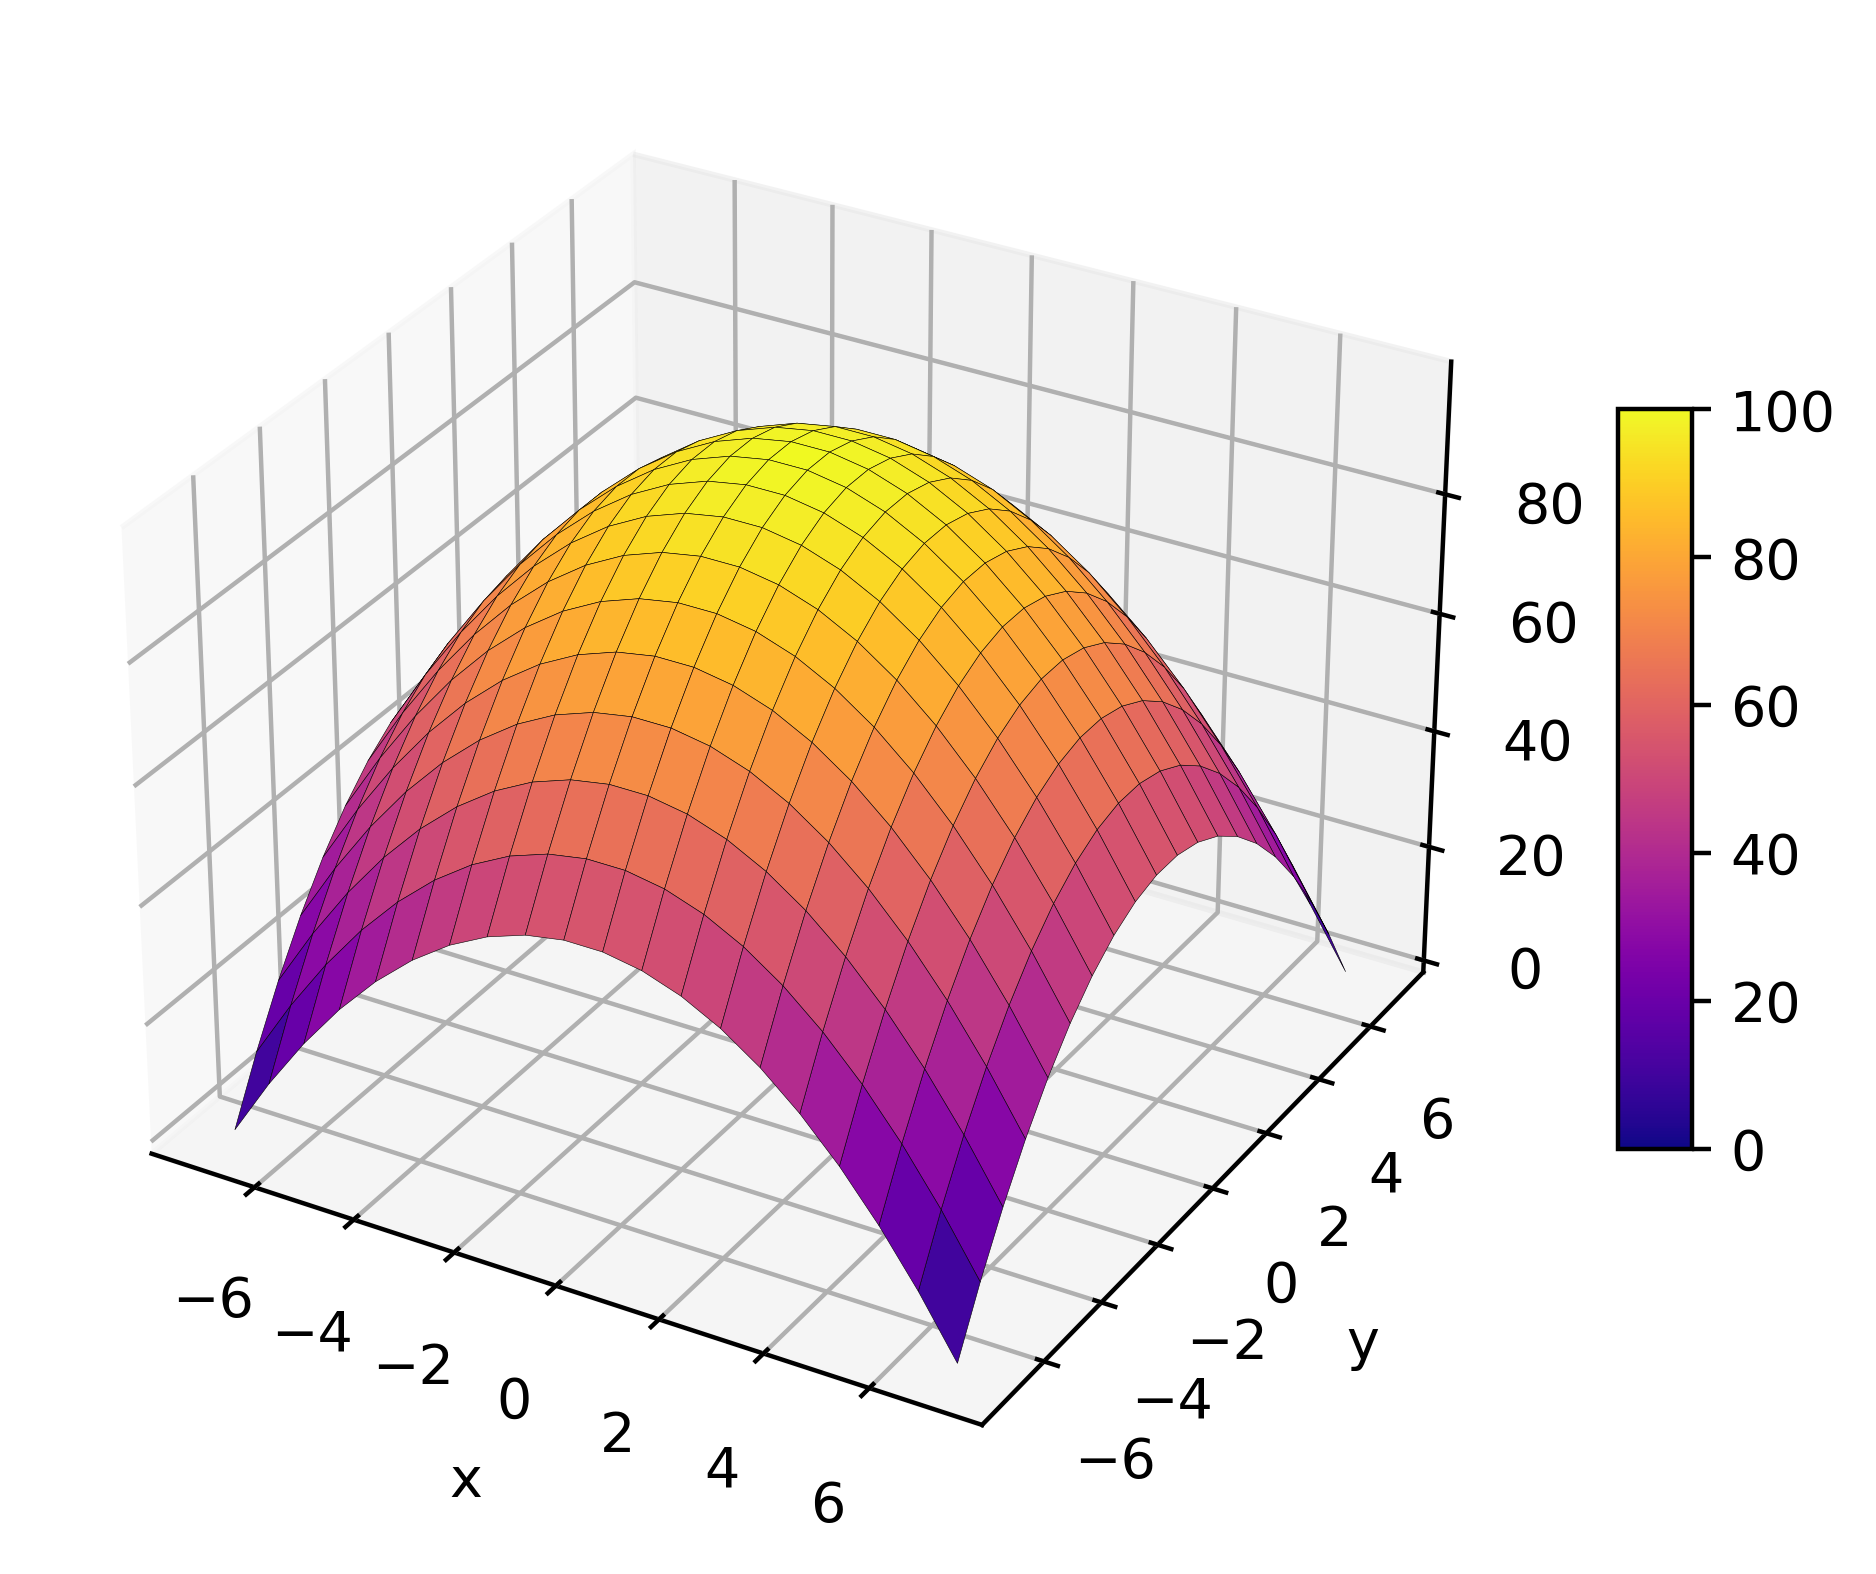
\includegraphics[scale=0.9]{figuras/der-parc2-1.png}
\end{minipage}
\begin{minipage}{0.4\textwidth}
	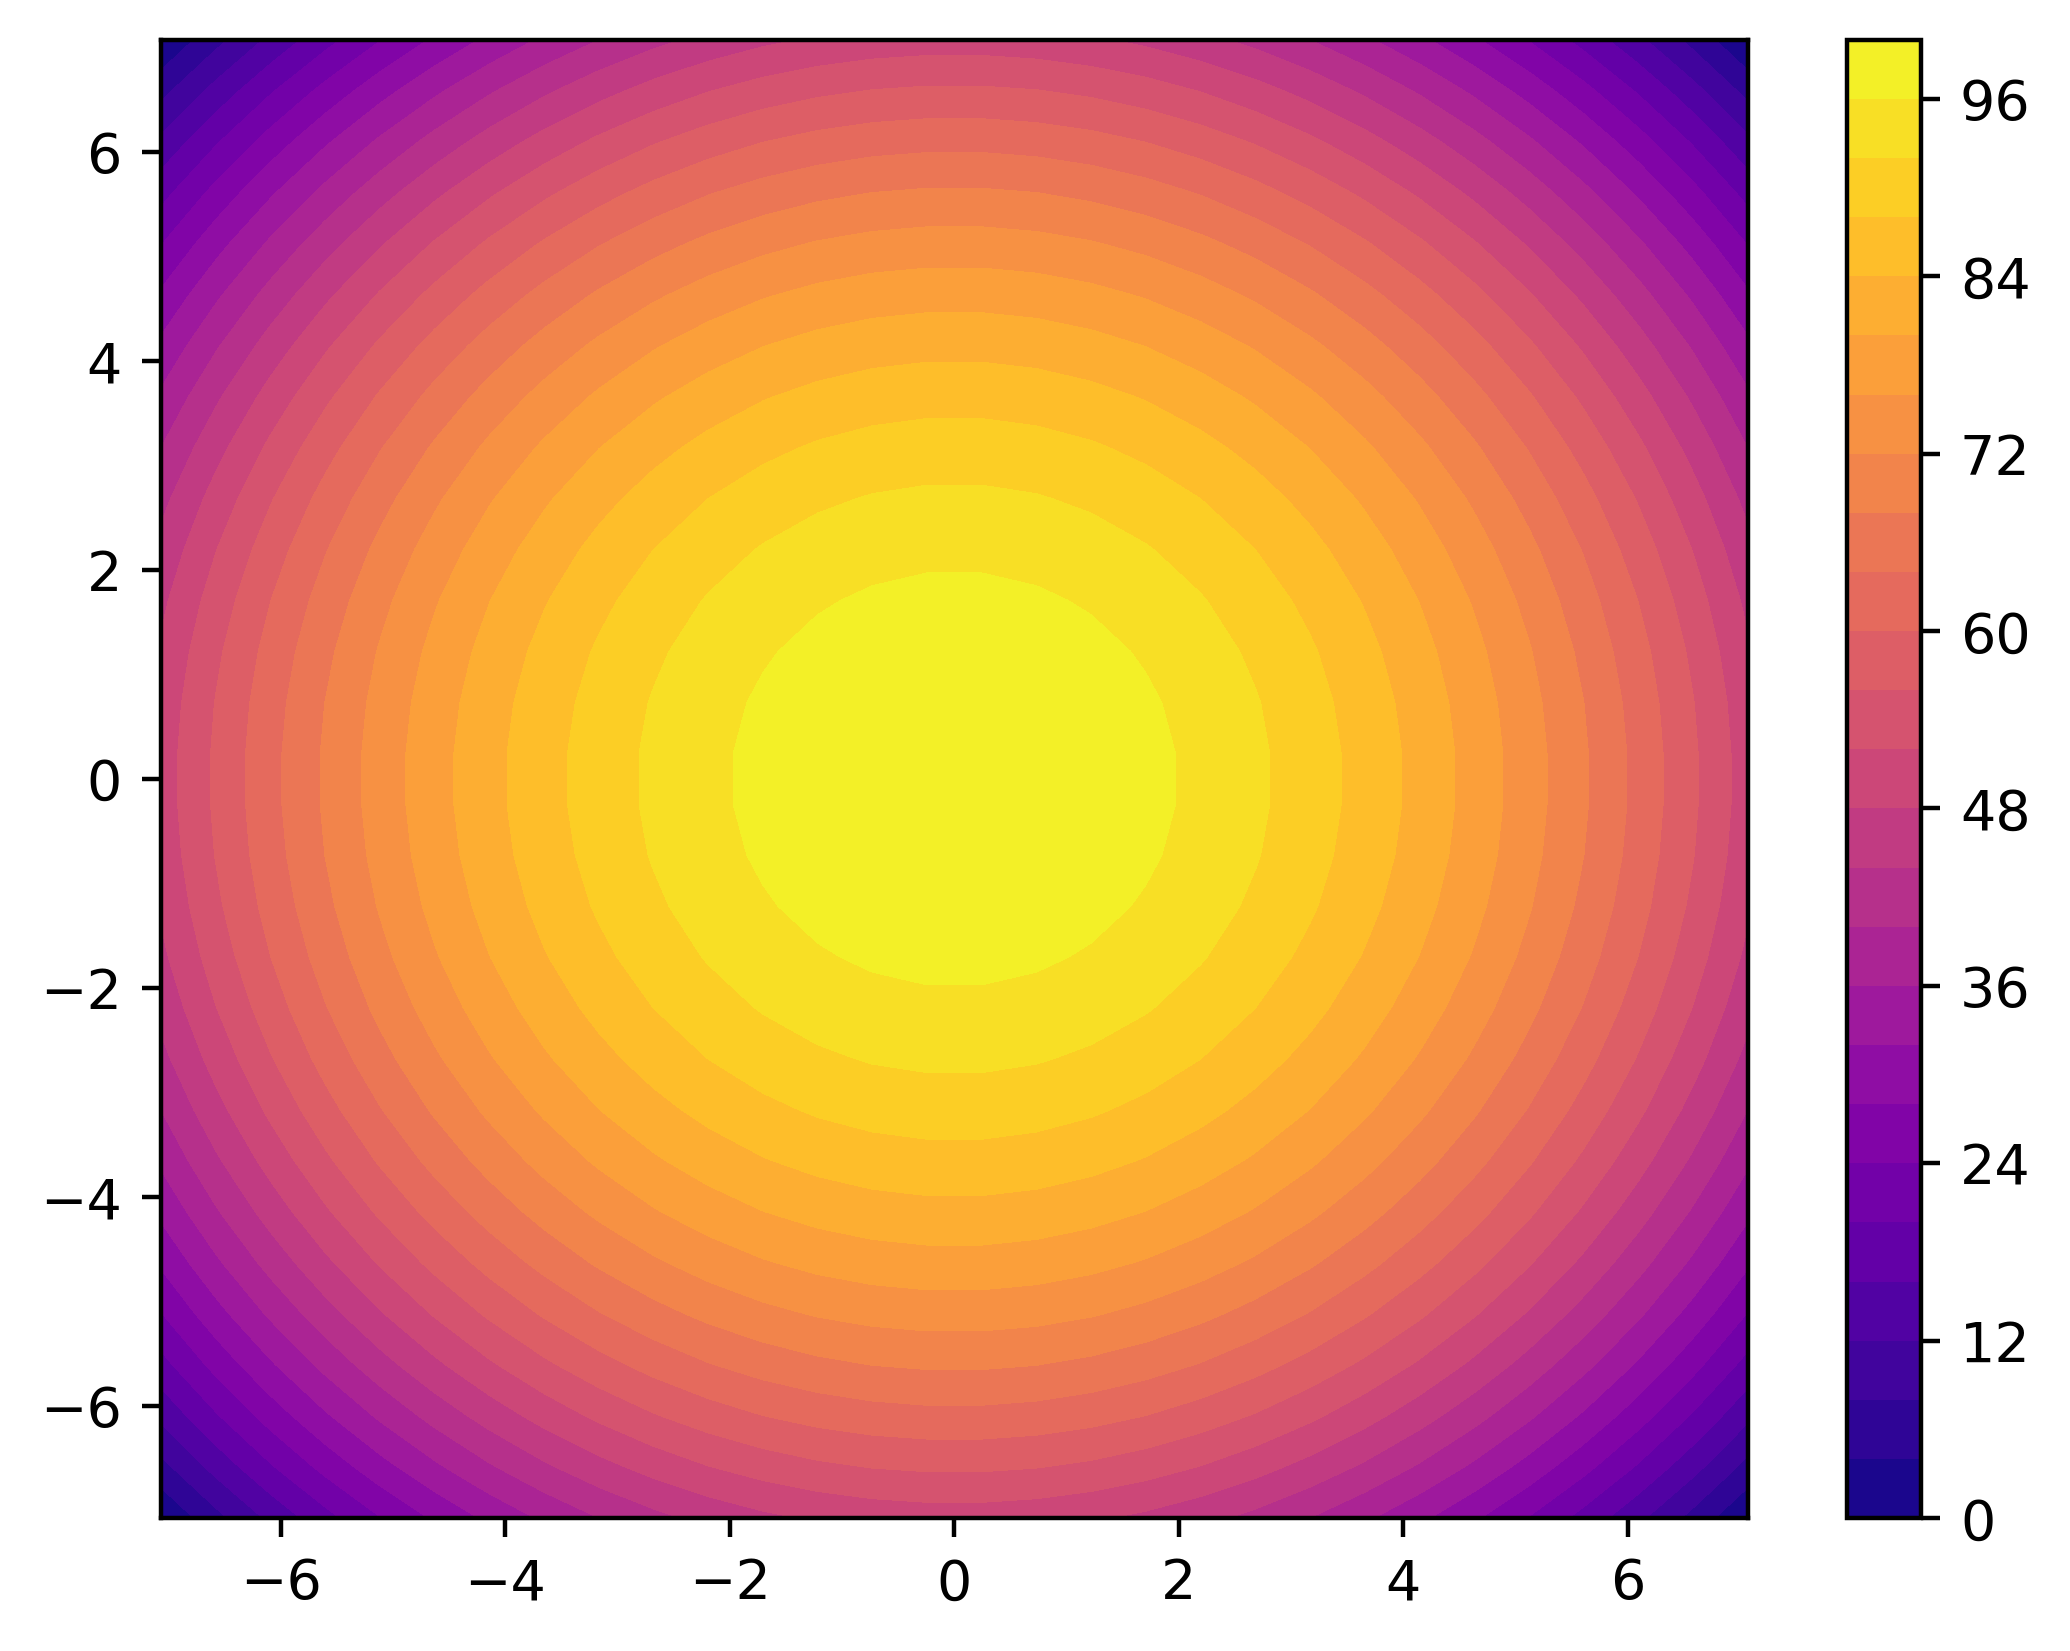
\includegraphics[scale=0.6]{figuras/der-parc2-1-nivel.png}
\end{minipage}
\end{center}

\begin{enumerate}
	\item Qual é a temperatura no ponto \(P=(2,-3)\)?
	\item Qual é a taxa de crescimento/decrescimento da temperatura no ponto \(P\) quando andamos na direção positiva de \(x\)? E na direção positiva de \(y\)?
\end{enumerate}
\newpage
\[
f_1({\color{red}x})=f({\color{red}x},-3)=91-{\color{red}x^2}, \ -5\sqrt{2}\leq {\color{red}x}\leq 5\sqrt{2} \]

\[f_2({\color{blue}y})=f(2,{\color{blue}y})=96-{\color{blue}y^2}, \ -5\sqrt{2}\leq {\color{blue}y}\leq 5\sqrt{2} \]

\begin{center}
	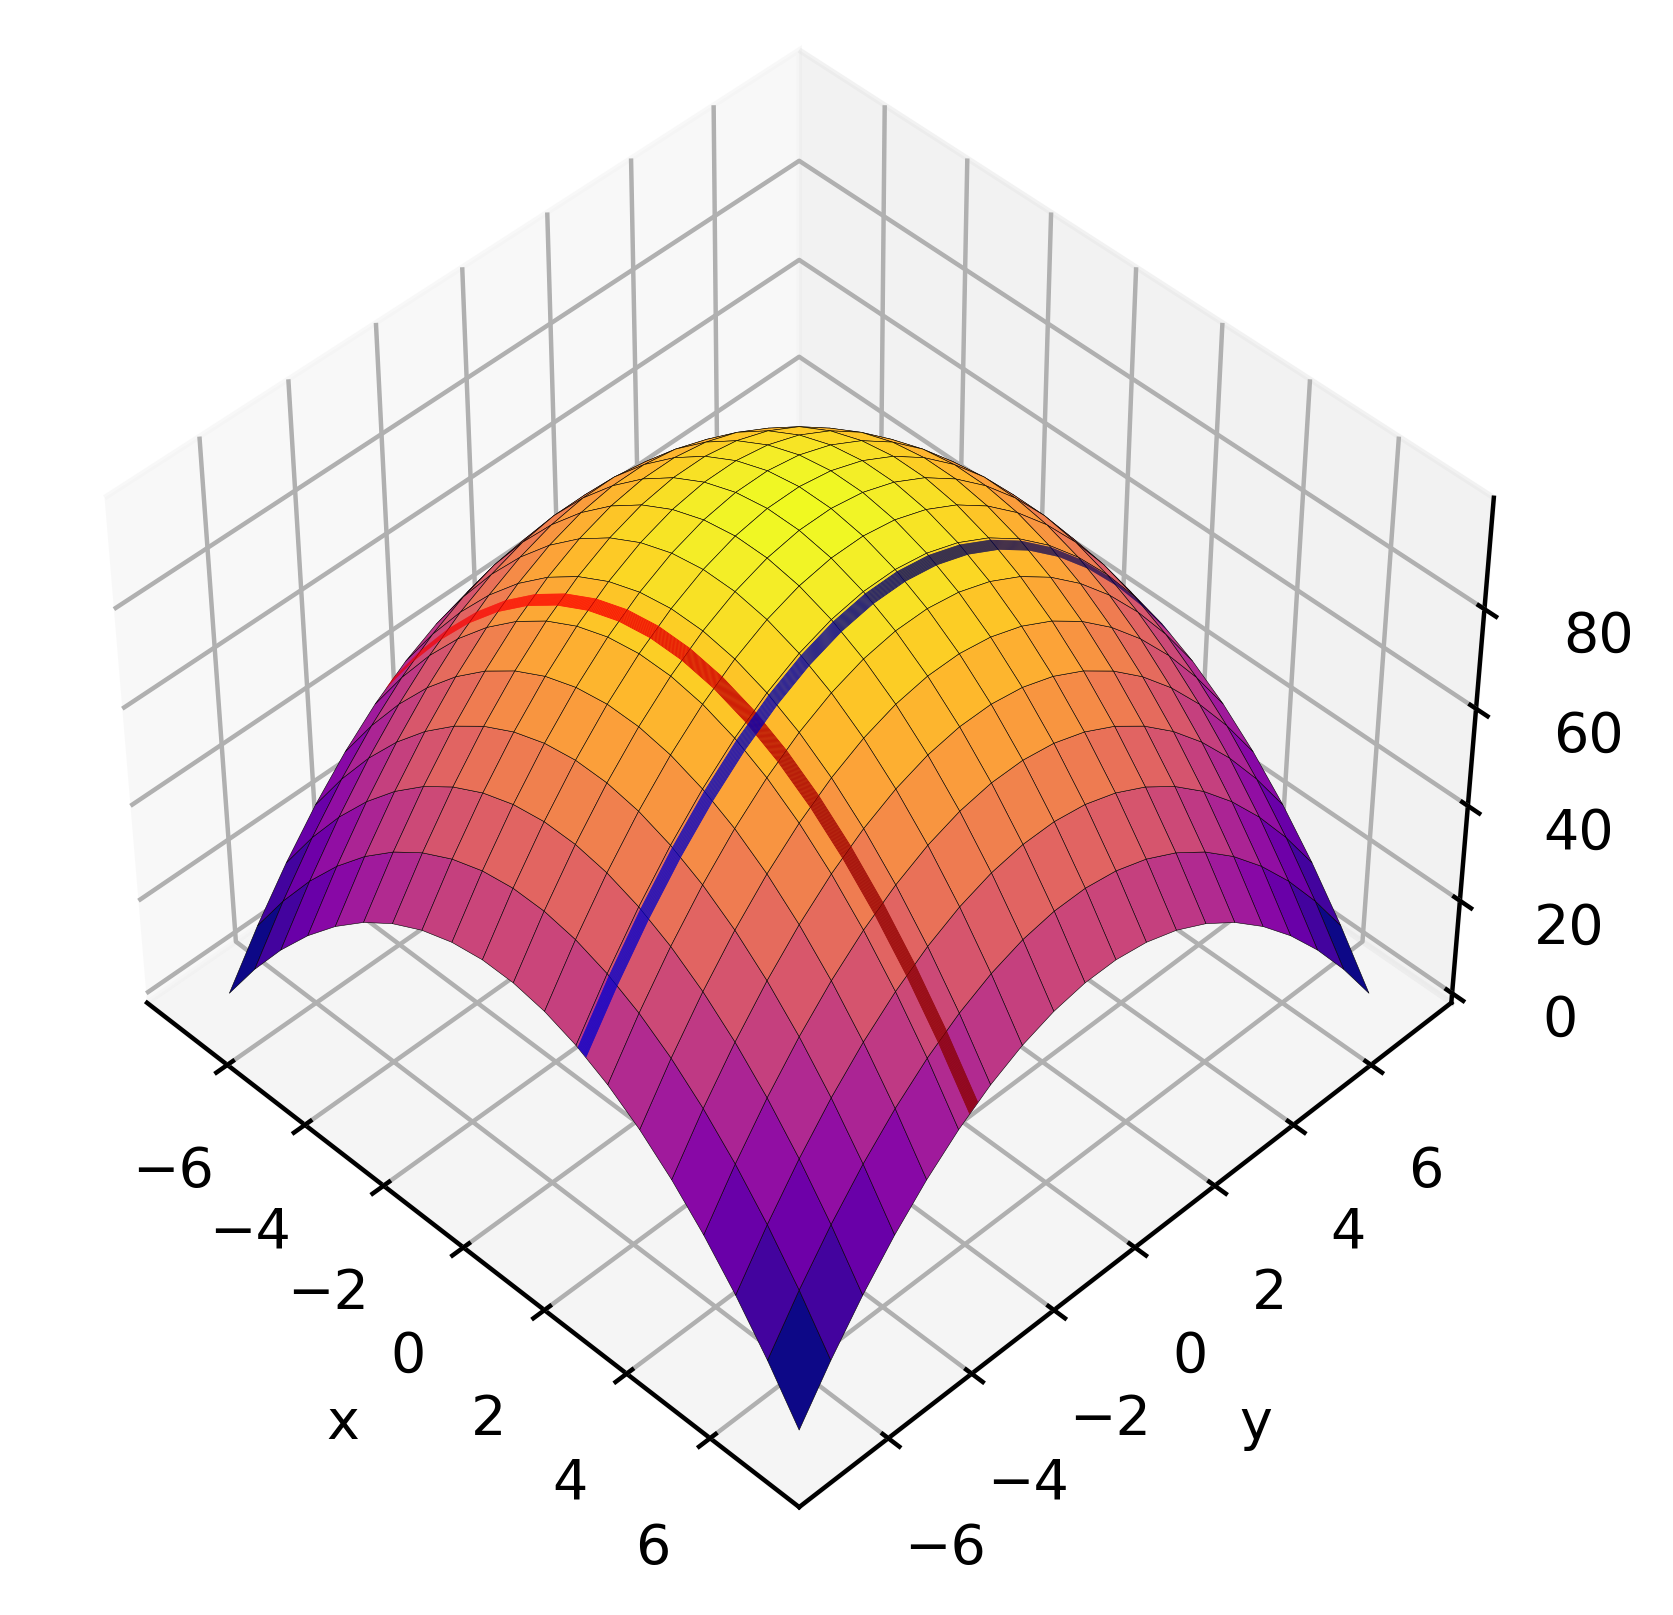
\includegraphics[scale=1]{figuras/der-parc2xy-2.png}
\end{center}

\begin{minipage}{0.45\textwidth}
A {\color{red}taxa de variação da temperatura}, no ponto $P=(2,-3)$, é de $-4^\circ C/m$ na {\color{blue}direção positiva do eixo $x$}. Em outras palavras, se caminharmos sobre a placa, a partir do ponto $P=(2,-3)$, {\color{blue}direção positiva do eixo $x$}, {\color{red}a temperatura vai cair a uma taxa de $-4^\circ C/m$.}
\end{minipage}
\begin{minipage}{0.45\textwidth}
\begin{center}
	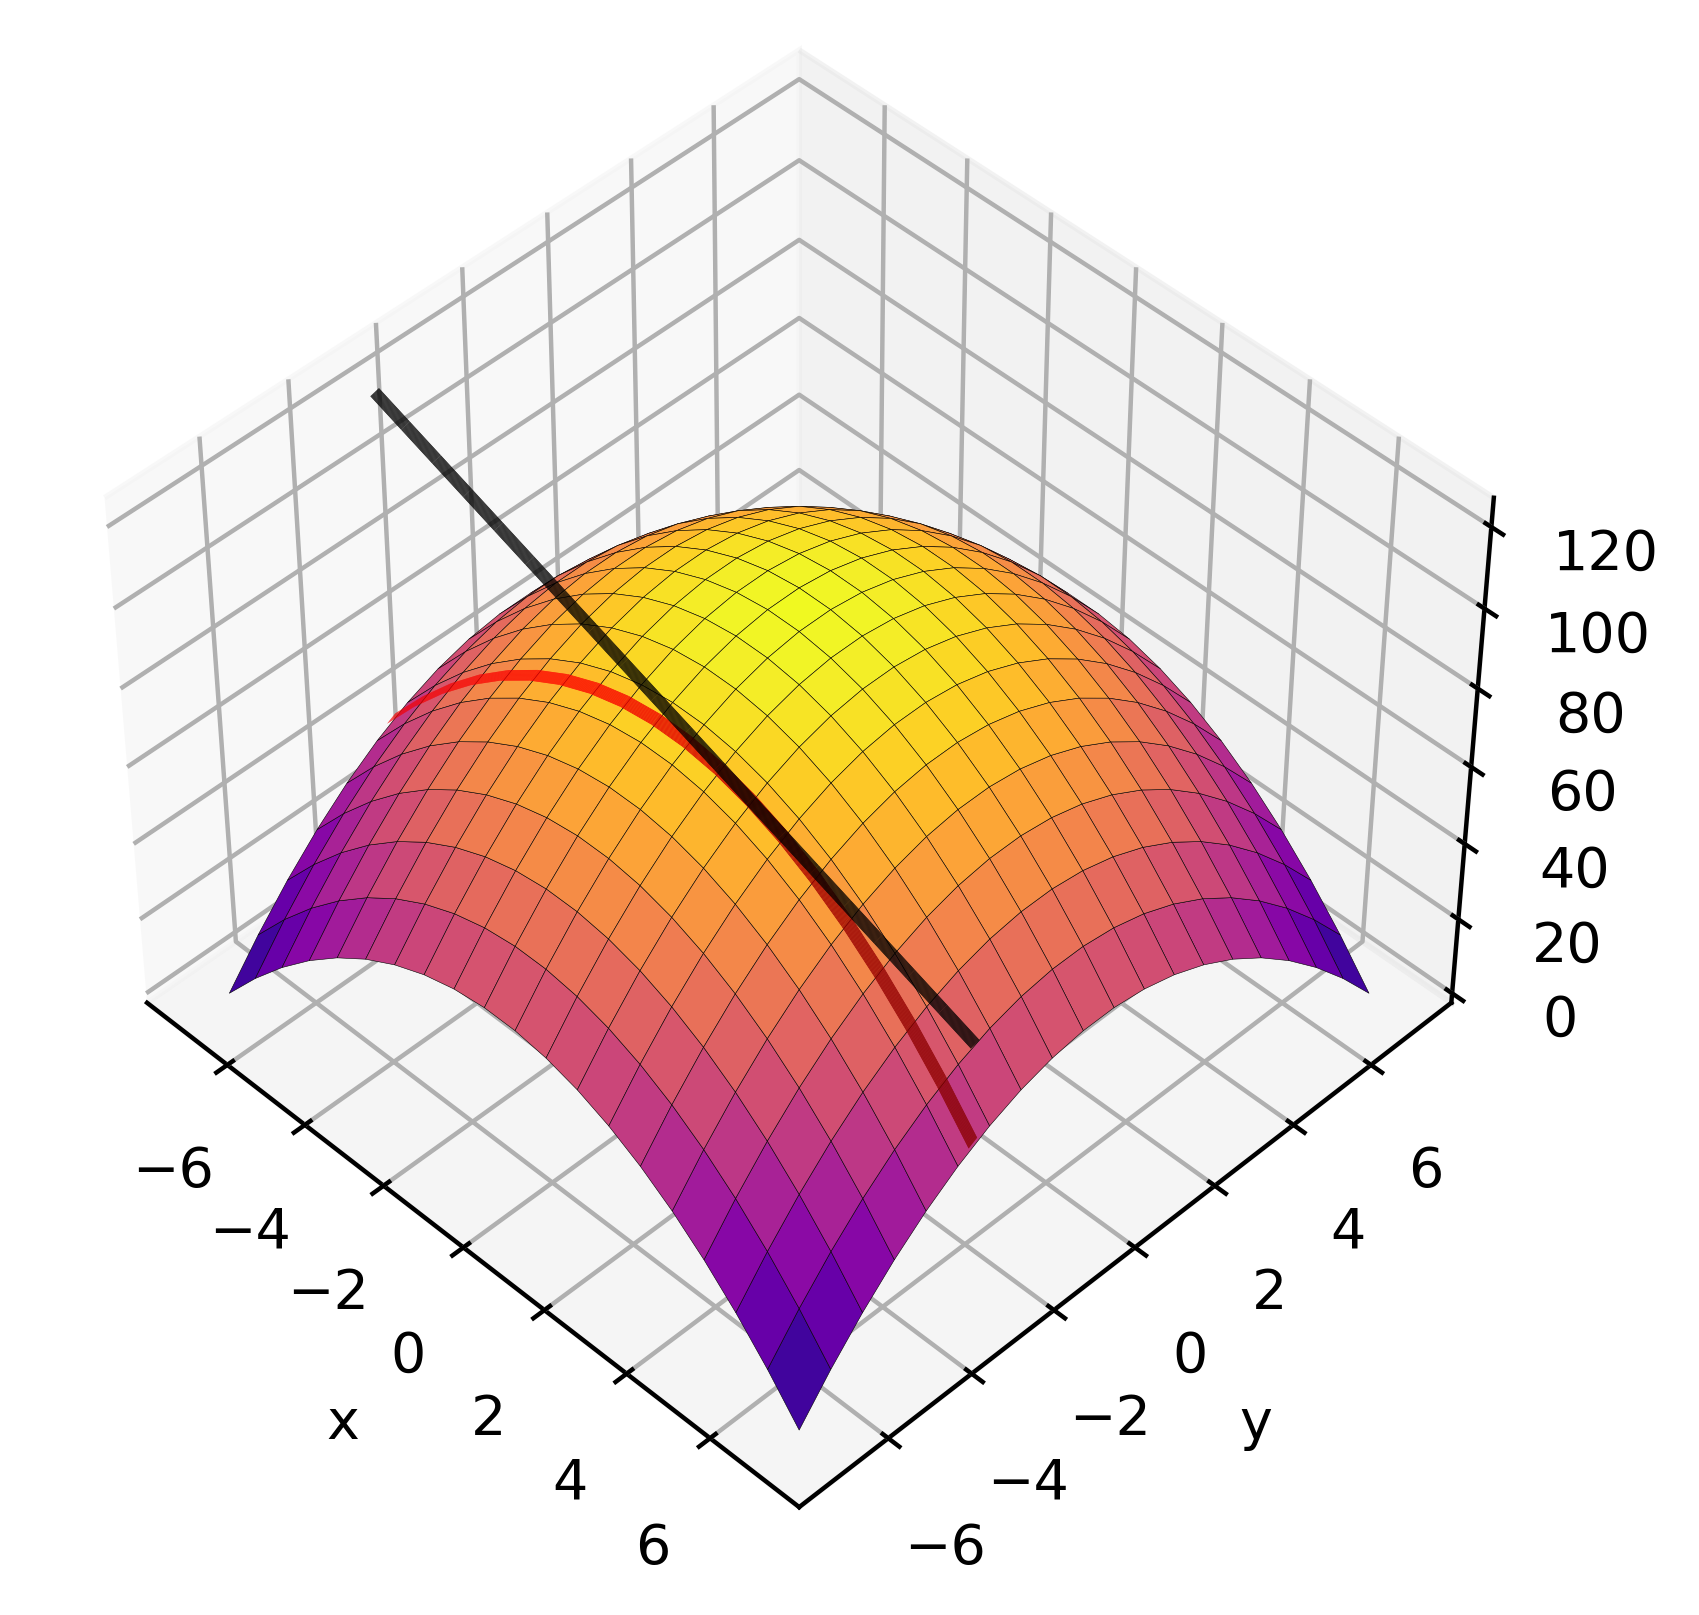
\includegraphics[scale=1]{figuras/der-parc2-3.png}
\end{center}
\end{minipage}
\newpage

\begin{definb}{}{}
 Sejam $f:U\subset\R^2\to \R$ uma função e $(a,b)\in U$. A \dt{derivada parcial de $f$ em relação a $x$} no ponto $(a,b)$ é dada por
$$\dx{f}(a,b)=\lim_{h\to 0}\frac{f(a+h,b)-f(a,b)}{h},$$
quando este limite existe. Analogamente, A \dt{derivada parcial de $f$ em relação a $y$} no ponto $(a,b)$ é dada por
$$\dy{f}(a,b)=\lim_{h\to 0}\frac{f(a,b+h)-f(a,b)}{h},$$
	quando este limite existe. 
\end{definb}

Analogamente se $f:U\subset\R^3\to \R$ uma função definida em um aberto $U$ contendo $(a,b,c)$. As derivadas parcial de $f$ em relação a $x$, $y$ e $z$  no ponto $(a,b,c)$ são dadas pelos limites
\[\dx{f}(a,b,c)=\lim_{h\to 0}\frac{f(a+h,b,c)-f(a,b,c)}{h},\]
\[\dy{f}(a,b,c)=\lim_{h\to 0}\frac{f(a,b+h,c)-f(a,b,c)}{h},\]
\[\dz{f}(a,b,c)=\lim_{h\to 0}\frac{f(a,b,c+h)-f(a,b,c)}{h},\]
quando estes limites existem. 

\begin{exeb}{}{}
	Se $f(x,y,z)=e^{xy}\log(z)$, determine as derivadas parciais.
\end{exeb}

\newpage

\begin{casab}{}{}
	\begin{enumerate}
		\item Se $f(x,y)=\sin\left(\frac{x}{1+y}\right)$, calcule $f_x$ e $f_y$.
		
		\item Se $f(x,y,z)=x\sin(y-z)$, determine as derivadas parciais.
	\end{enumerate}
\end{casab}

\marcador{subsection}{Derivadas de Ordem superior}

Se $z=f(x,y)$ é uma função, então  $\dx{f}$ e $\dy{f}$ também são funções de duas variáveis e portanto  podemos definir quatro novas funções que são chamadas de \dt{derivadas parciais de segunda ordem de f}, a saber:
\begin{multicols}{2}
$\displaystyle f_{xx}=\frac{\partial^2f}{\partial x^2}=\dx{}\left(\dx{f}\right)$

$\displaystyle f_{xy}=\frac{\partial^2f}{\partial y\partial x}=\dy{ }\left(\dx{f}\right)$
		
		
$\displaystyle f_{yx}=\frac{\partial^2f}{\partial x\partial y}=\dx{}\left(\dy{f}\right)$
	
$\displaystyle f_{yy}=\frac{\partial^2f}{\partial y^2}=\dy{}\left(\dy{f}\right)$

\end{multicols}

\begin{exeb}{}{} Calcule todas as derivadas parciais de segunda ordem da função $f(x,y)=x^3+x^2y^3-2y^2$.
\end{exeb}


\vfill

\begin{theoremb}{}{} Se $z=f(x,y)$ é de classe $C^2$, então suas derivadas mistas são iguais, isto é, 
	$$\frac{\partial^2 f}{\partial x\partial y}=\frac{\partial^2 f}{\partial y\partial x}.$$
\end{theoremb} 



